\section{Results}
This section emphasize the advantages of EMD to efectively uncover correlated signals/sensors(?).
First, we demonstrate the benefit of EMD with a simple example, the three sensorsr presented in Section \ref{problem}.
Second, we validate the proposed methodology with a large dataset (674 sensors) and highlight that EMD uncovers the spatial correlation of the sensors.

\subsection{Simple Scenario}
Lets consider the simple example of Section \ref{problem} where we would like to know if an EHP signal is correlated with the two other signals; a light signal and a GHP signal.
Using the raw signals, the correlation coefficients suggest that the light and GHP signals are both correlated to the EHP signal (Table \ref{tab:corr}).
As stated in previous section this result is certainly biased by the strong daily pattern shared by these three signals.

Extracting the weekly pattern of the data using EMD permits a more detailed analysis of these signals.
Figure \ref{fig:emd} depicts the EMD decomposition of the three signals.
Notice that the EMD process has been stopped once the daily pattern have been uncovered.
Thereby, for each signal EMD has retrieved three IMFs that highlight the high frequency characteristics of the signals.

The correlation coefficients for the EHP and light IMFs --- i.e. $0.4431$, $0.5104$ and $0.6171$ corresponding respectively to the IMF1, IMF2 and IMF3 --- emphasize the positive correlation of the two signals in the high frequency domain.
However, the correlation coefficients for the EHP and GHP IMFs show that the two signals are independent in the high frequency domain.
Therefore, EMD allow us to effectively identify that the light signal is related to the EHP whereas the GHP one is not.


\begin{table*}
\begin{center}
\begin{tabular}{|l|l|l|l|l|l|}
\hline
× & Raw signal & 1st IMF & 2nd IMF & 3rd IMF & Residual\\ \hline
EHP, Light & 0.7720 & 0.4431 & 0.5104 & 0.6171 & 0.8114\\ \hline
EHP, GHP & 0.6369 & -0.0055 & 0.0883 & 0.2350 & 0.7956\\ \hline
\end{tabular}
\caption{Correlation coefficients of the analyzed signal and their IMFs uncovered by EMD}
\label{tab:corr}
\end{center}
\end{table*}


\subsection{Validation}
\begin{figure*}
\centering
 \subfigure[Raw signals correlation coefficients]{\label{fig:histo1}\includegraphics[width=.45\textwidth]{img/allFloors_week1_week4_corr_abs.eps}}
 \subfigure[Average IMFs correlation coefficients]{\label{fig:histo2}\includegraphics[width=.45\textwidth]{img/allFloors_week1_week4_emd_abs.eps}}
 \caption{Distribution of the correlation coefficients of the raw signals and corresponding IMFs using 3 weeks of data from 674 sensors deployed on 12 Floors.}
\label{fig:histo}
\end{figure*}

In order to validate the effectiveness of the proposed approach to identify correlated signals, we analyze three week signals from the 674 sensors deployed in the building.
For each signal $S$ we compute the correlation coefficient for $S$ and the EHP signal and the average value of the IMFs correlation coefficients obtained with EMD.
Figure \ref{fig:histo1} shows the distribution of the raw signal correlation coefficients.
Regarding this figure a large fraction of the dataset seems to be correlated with the EHP signal.
Indeed half of the analyzed signals provide a correlation coefficient higher than $0.36$.
Although the highest score correspond to the light signal that is actually from the same room as the EHP signal, all signals that achieve a score higher than $0.6$  correspond to 118 heat pumps that are located at different floors and are independent from the analyzed EHP signal.
Moreover, the distribution of the signals is almost uniform, thus, discriminating signals correlated to the analyzed one is a laborious task.

Figure \ref{fig:histo2} shows the distribution of the average correlation coefficients for the IMFs of each signal and the analyzed EHP one.
Here the number of signals correlated to the analyzed one is significantly small. 
Only 10 signals perform a score higher than $0.25$ and their distribution allow us to easily rank signals in term of correlation.

Interestingly the IMFs correlation coefficient reveal the spatial correlation of the sensors.
Figure \ref{fig:map} is the map floor where the EHP signal is measured.
The EHP sensors is located in the room $C2$.
The signal performing the highest score (i.e. $0.522$) is the light signal from the same room.
The two highest score for this floor (i.e. $0.316$ and $0.279$) are the light and EHP signals from next door, room $C1$.
% in the simple scenario the GHP is located in the room A5.

\begin{figure}
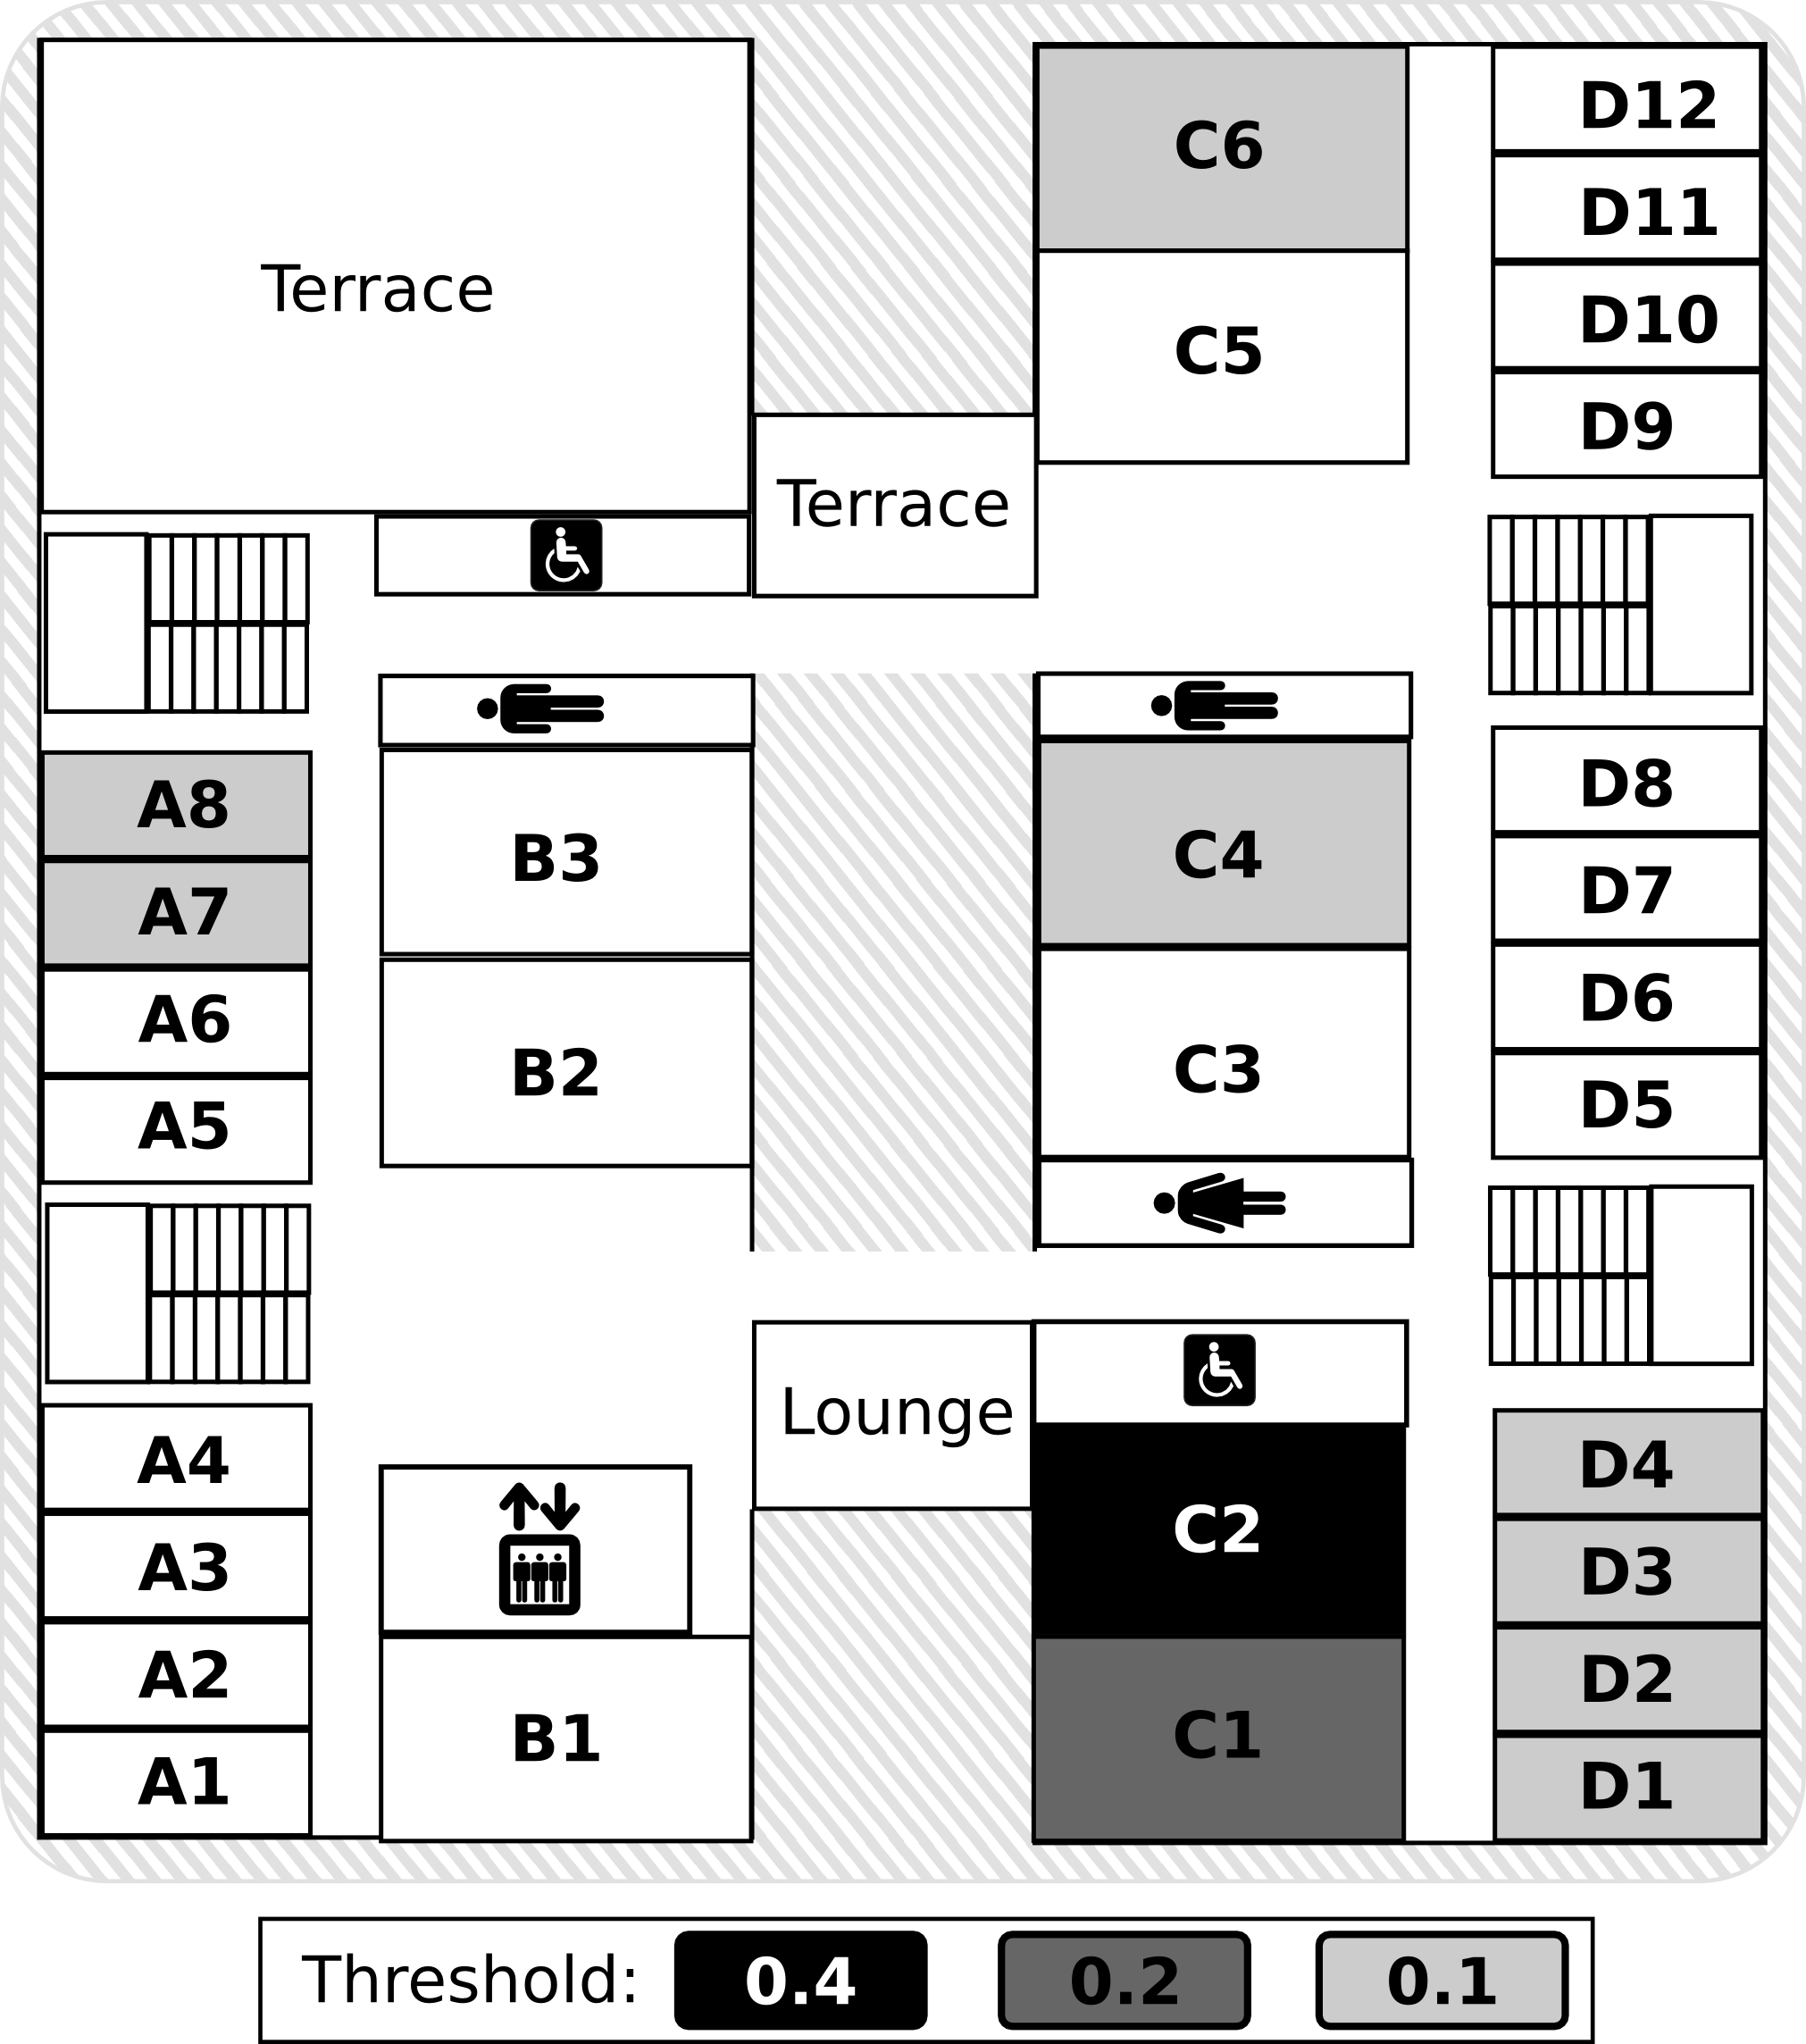
\includegraphics[width=.5\textwidth]{img/floorMap.png}
\caption{}
\label{fig:map}
\end{figure}
